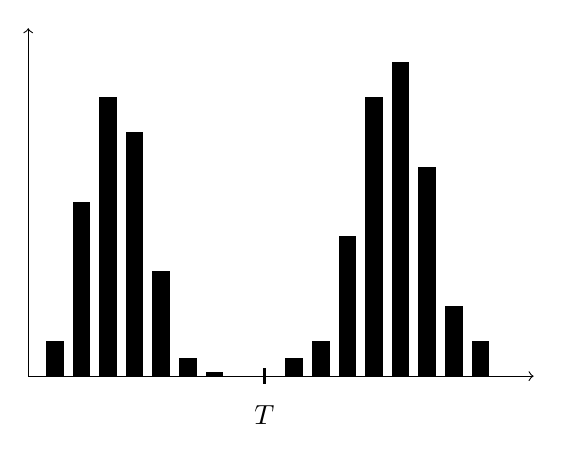
\begin{tikzpicture}
	\begin{axis}[
	            xtick=data,
	            axis x line = bottom,
	            axis y line = left,
	            axis line style={->},
	            xtick=\empty,
	            ytick=\empty,
	            ymin = 0,
	            ymax = 100,
	            xmin = 0,
	            xmax = 19,
	            bar width=6pt,
	            height=6cm,
	            width=8cm
	          ]
	            \addplot[ybar,fill=black] coordinates {
	                (1,10)
	                (2,50)
	                (3,80)
	                (4,70)
	                (5,30)
	                (6,5)
	                (7,1)
	                (8,0)
	                (9,0)
	                (10,5)
	                (11,10)
	                (12,40)
	                (13,80)
	                (14,90)
	                (15,60)
	                (16,20)
	                (17,10)
	            };
	\end{axis}
	
	\draw[thick] (3,0.1) -- (3,-0.1);
	\node at (3,-0.5) {$T$};
\end{tikzpicture}